\vspace{2cm}

\begin{center}
\begin{Huge}
\textbf{Änderung}
\end{Huge}
\end{center}
Das Lastenheft, welches bei der Projektgenehmigung mit eingereicht wurde, weißt einen Fehler auf. 
\\
Es war zu jedem Zeitpunkt zwischen mir und meinem Auftraggeber klar, dass von meiner Seite aus, ein Prototyp entwickelt werden soll. Eine Lebenszeitberechnung für ein noch nicht fertiggestelltes Produkt ist daher nicht sinnvoll.
\\
In der ersten Version des Lastenheftes, wurde dieses Detail leider nicht schriftlich festgehalten. Dies hat sich in meiner nun folgenden Dokumentation geändert.



\vspace{5cm}

\begin{Huge}
\begin{center}
\textbf{Wichtige Anmerkung}
\end{center}
\end{Huge}
Bei der vorliegenden Dokumentation handelt es sich um eine umfassende Dokumentation zu meinem Projekt. 
\\
Diese beinhaltet in kombinierter Form die Dokumentation für die IHK und meinem Auftraggeber.
\\
Die mit transparenter blauer Farbe markierten Abschnitte sind für die IHK-Abschlussprüfung relevant. 
\\
Die mit transparenter roter Farbe markierten Abschnitte sind die nicht für die IHK relevanten Dokumentationsteile. Sie sind von meinem Auftraggeber gefordert und sollen dem Prüfungsausschuss nur zum Verständnis dienen.

\newpage

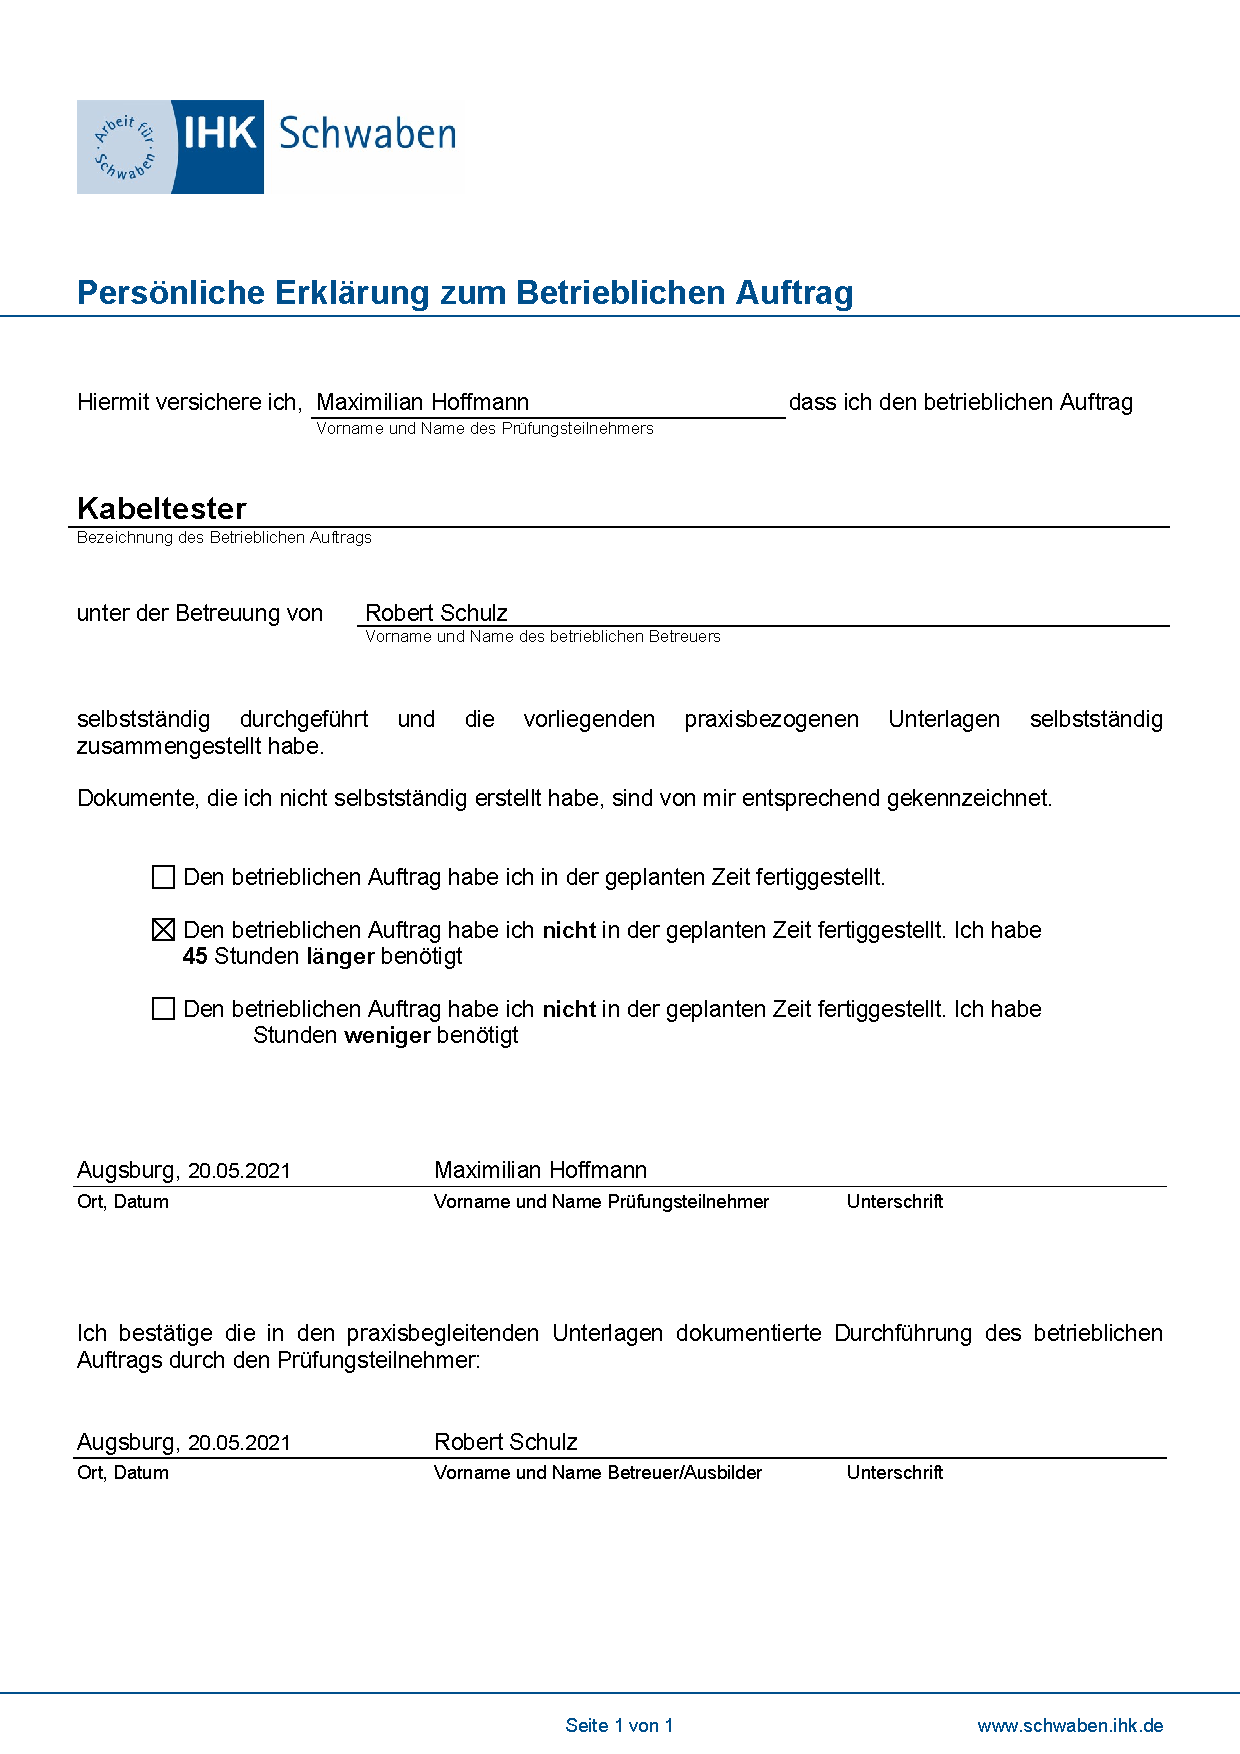
\includepdf[pages = 1] {PDF/BA_Persoenliche.pdf}



